\documentclass[usepdftitle=false]{beamer}

\usetheme{Boadilla}
\usefonttheme{professionalfonts}
\setbeamertemplate{navigation symbols}{}

%
% Packages
%

\usepackage{fontspec}
\usepackage[english]{babel}
\usepackage[babel, final]{microtype}

\usepackage{mathtools}
\usepackage{amsthm}
\usepackage{unicode-math}
\usepackage[ruled, longend]{algorithm2e}
\usepackage{prftree}

\usepackage{fancyvrb}
\usepackage[newfloat]{minted}

\usepackage{booktabs}
\usepackage{graphicx}
\usepackage[compatibility=false]{caption}
\usepackage{subcaption}

\usepackage{tikz}
\usepackage{tikzpeople}
\usepackage{pgfplots}
\usepackage{pgfplotstable}

\usepackage[strict, autopunct]{csquotes}
\usepackage[hyperref, backend=biber, maxcitenames=2, giveninits]{biblatex}

\usepackage{siunitx}
\usepackage{nth}

\usepackage[shortcuts]{extdash}

%
% Setup
%

\defaultfontfeatures{Ligatures=TeX}
\addbibresource{\jobname.bib}
\unimathsetup{%
  math-style=ISO,
  bold-style=ISO%
}
\mathtoolsset{
  mathic%
}
\sisetup{%
  detect-all,
  detect-display-math,
  binary-units%
}
\hypersetup{%
  unicode,
  breaklinks,
  pdftitle={Error-Correcting Codes in the Rank Metric},
  pdfauthor={Dario Gjorgjevski},
  pdfsubject={Bachelor's Thesis},
  pdfkeywords={Coding Theory, Cryptography}%
}
\pgfplotsset{compat=newest}
\usetikzlibrary{calc, positioning, shapes}



%
% Commands
%

% Notation from linear algebra
\AtBeginDocument{%
  \renewcommand*{\vec}{\symbf}
  \newcommand*{\mat}{\symbf}
  \newcommand*{\trans}{\top}%
}
\DeclareMathOperator{\rank}{rank}
\DeclareMathOperator{\lspan}{span}
\DeclareMathOperator{\supp}{supp}
\DeclarePairedDelimiter{\basis}{\langle}{\rangle}
\newcommand*{\M}{\ensuremath{\mathcal{M}}}
\newcommand*{\GL}{\ensuremath{\mathsf{GL}}}

% Notation from probability and statistics
\DeclareMathOperator{\E}{E}
\DeclareMathOperator{\var}{var}
\DeclareMathOperator{\cov}{cov}

% Notation from cryptography
\newcommand*{\pub}{\ensuremath{\mathsf{pub}}}
\newcommand*{\priv}{\ensuremath{\mathsf{priv}}}
\newcommand*{\enc}{\ensuremath{\mathsf{Enc}}}
\newcommand*{\dec}{\ensuremath{\mathsf{Dec}}}

% Standard sets
\newcommand*{\KK}{\ensuremath{\mathbb{K}}}
\newcommand*{\FF}{\ensuremath{\mathbb{F}}}
\newcommand*{\NN}{\ensuremath{\mathbb{N}}}
\newcommand*{\ZZ}{\ensuremath{\mathbb{Z}}}
\newcommand*{\RR}{\ensuremath{\mathbb{R}}}
\newcommand*{\CC}{\ensuremath{\mathbb{C}}}

% Complexity classes
\newcommand*{\NP}{\ensuremath{\mathcal{NP}}}

% Asymptotic notation
\newcommand*{\BigOh}{\mathcal{O}}

% Linear codes
\newcommand*{\Gop}{\ensuremath{\Gamma}}
\newcommand*{\Gab}{\ensuremath{\mathfrak{G}}}

% arg{min,max}
\DeclareMathOperator*{\argmin}{arg\,min}
\DeclareMathOperator*{\argmax}{arg\,max}

% Sampling
\newcommand*{\sample}{\ensuremath{\gets_{\mathrm{\$}}}}

% Computational problems
\newcommand*{\MDD}{\ensuremath{\mathsf{MDD}}}
\newcommand*{\CSD}{\ensuremath{\mathsf{CSD}}}
\newcommand*{\SW}{\ensuremath{\mathsf{SW}}}
\newcommand*{\MR}{\ensuremath{\mathsf{MR}}}

% Ceiling and floor
\DeclarePairedDelimiter{\floor}{\lfloor}{\rfloor}
\DeclarePairedDelimiter{\ceil}{\lceil}{\rceil}

% Absolute value and norm
\DeclarePairedDelimiter{\abs}{\lvert}{\rvert}
\DeclarePairedDelimiter{\norm}{\lVert}{\rVert}

% Custom norms and distances
\newcommand*{\normH}[1]{\ensuremath{\norm{#1}_{\mathrm{H}}}}
\newcommand*{\normR}[2]{\ensuremath{\norm{#1}_{#2}}}
\DeclareMathOperator{\dH}{d_H}
\DeclareMathOperator{\dR}{d_R}

% Set cardinality
\DeclarePairedDelimiter{\card}{\lvert}{\rvert}

% Gaussian binomial coefficient
\DeclareRobustCommand{\qbinom}{\genfrac[]{0pt}{}}

% Miscellaneous notation
\newcommand*{\sys}{\ensuremath{\mathsf{sys}}}
\newcommand*{\ext}{\ensuremath{\mathsf{ext}}}
\newcommand*{\reg}{\ensuremath{\mathsf{reg}}}

\newcommand*{\KS}{\ensuremath{\mathsf{KS}}}
\newcommand*{\GV}{\ensuremath{\mathsf{GV}}}
\newcommand*{\LB}{\ensuremath{\mathsf{LB}}}

\newcommand*{\Distort}{\mathcal{D}}

\newcommand*{\PlainISD}{\textsc{Plain}\=/ISD}
\newcommand*{\LBISD}{LB\=/ISD}

%
% Title
%

\title{Error\-/Correcting Codes in the Rank Metric}
\subtitle{With Applications to Cryptography}
\author[Dario Gj.]{%
  Dario Gjorgjevski\inst{1}\\%
  \href{mailto:gjorgjevski.dario@students.finki.ukim.mk}%
  {\nolinkurl{gjorgjevski.dario@students.finki.ukim.mk}}
}
\institute[FCSE]{%
  \inst{1}Faculty of Computer Science and Engineering\\%
  Ss.\ Cyril and Methodius University in Skopje
}
\date{January 30, 2018}


%
% Logo
%

%\logo{
\includegraphics[height=0.66cm]{../Logo_ФИНКИ.pdf}}


%
% Table of contents
%

\AtBeginSection[]{%
  \begin{frame}{Contents}
    \tableofcontents[hideothersubsections]
  \end{frame}%
}

%
% Document
%

\begin{document}

\begin{frame}
  \titlepage
\end{frame}

\section{Introduction}

\subsection{Crash Course in Cryptography}

\begin{frame}{Past vs.\ Present}
  \begin{itemize}
  \item In the past, cryptography was used to provide secure
    communication in an \emph{ad\-/hoc manner}.
  \item This picture changed radically with the development of a rich
    and rigorous theory in the late \nth{20} century.
  \item Today, we have algorithms for secure communication in two
    settings: \emph{\alert{symmetric}} and \emph{\alert{asymmetric}}.
  \item We will quickly review both; however, the remainder of this
    thesis focuses entirely on algorithms for secure communication in
    the asymmetric setting.
  \end{itemize}
\end{frame}

\begin{frame}{The Symmetric Setting}
  \begin{itemize}
  \item The message \(m\) is \emph{encrypted} under the secret key
    \(k\) to obtain the \emph{ciphertext} \(c\).
  \item The ciphertext \(c\) is \emph{decrypted} under \alert{the same
      key} \(k\).
  \item If the two parties could share the secret key securely, why
    could they not do the same with the message?
  \end{itemize}
  \begin{figure}
    \centering
    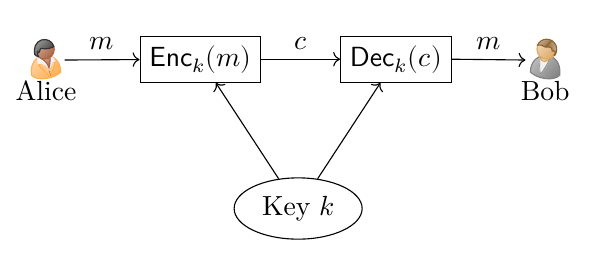
\begin{tikzpicture}
      \node[alice] (alice) {Alice};
      \node[draw, right=of alice] (encryption) {\(\enc_k(m)\)} edge[<-] node[above] {\(m\)} (alice);
      \node[draw, right=of encryption] (decryption) {\(\dec_k(c)\)} edge[<-] node[above] {\(c\)} (encryption);
      \node[bob, right=of decryption, mirrored] (bob) {Bob} edge[<-] node[above] {\(m\)} (decryption);
      \coordinate (center) at ($(encryption)!0.5!(decryption)$);
      \node[draw, ellipse, below=1.5cm of center] (key) {Key \(k\)} edge[->] (encryption) edge[->] (decryption);
    \end{tikzpicture}
    \caption{Secure communication in the symmetric setting.}
  \end{figure}
\end{frame}

\begin{frame}{The Asymmetric Setting}
  Cryptography in the asymmetric setting is called \emph{public\-/key
    cryptography}.  The RSA (\textcite{RSA78}) cryptosystem is the
  most widely used and one of the first asymmetric cryptosystems:
  \begin{enumerate}
  \item Encryption is done with the intended recipient's \emph{public
      key}, \(k_{\pub}\), known to everybody.
  \item Decryption is done with the \emph{private key}, \(k_{\priv}\),
    known only to the recipient.
  \end{enumerate}
  \begin{block}{Real\-/world analogy}
    Think of a mailbox: encryption corresponds to leaving mail in a
    person's mailbox, decryption to the person opening the mailbox to
    retrieve it.
  \end{block}
\end{frame}

\begin{frame}{RSA Basics}
  RSA relies on the computational complexity of \emph{integer
    factorization}.
  \begin{example}[Integer factorization]
    If you were asked to multiply
    \[
      \num{17627949842247424607} \times \num{15969639761398924673}\text,
    \]
    you would need several minutes with pen and paper to arrive at
    \num{281512008712700373730275954373439628511}.  But, what if you
    were asked to find two integers, \(p\) and \(q\), such that
    \[
      p \times q = \num{281512008712700373730275954373439628511}\text?
    \]
  \end{example}
  Unfortunately, \textcite{Sho97} published an algorithm that can
  factor integers efficiently and hence \enquote{break} RSA\@.  The
  only drawback: it needs a \alert{quantum computer}.
\end{frame}

\subsection{Going Post-Quantum}

\begin{frame}{The McEliece Cryptosystem}
  \begin{itemize}
  \item A cryptosystem from roughly the same time as RSA is believed
    to be hard even for quantum computers: the McEliece cryptosystem.
  \item It relies on the hardness of decoding random codes over
    \(\FF_q\) in the Hamming metric.
  \item The problem was proven \NP\=/complete when \(q = 2\) by
    \textcite{BEvT78}; and in the general case by \textcite{Bar94}.
  \item The best attacks against McEliece come from a family of
    algorithms called \emph{information set decoding} (ISD).
  \end{itemize}
\end{frame}

\begin{frame}{Issues with McEliece}{\ldots{}and Fixing Them}
  \begin{itemize}
  \item Unfortunately, McEliece requires a key size of roughly
    \SI{192}{\kilo\byte} to achieve \num{128}\=/bit security against
    information set decoding \(\implies\) very prohibitive for
    embedded devices.
  \item \Textcite{GPT91} proposed the GPT cryptosystem which uses
    error\-/correcting codes in the \emph{rank metric}, as opposed to
    McEliece's Goppa codes which correct errors in the Hamming metric.
  \item GPT is believed to require much smaller keys in order to
    achieve the same security.
  \end{itemize}
\end{frame}

\subsection{Code-Based Cryptography}

\begin{frame}{Cryptography and the Information Transmission Model}
  \begin{itemize}
  \item The information transmission model comes from the landmark
    work of \textcite{Sha48}.
  \item It can be utilized for cryptographic purposes by means of
    error\-/correcting codes.  McEliece is one of the most prominent
    examples of such \emph{code\-/based cryptography}.
  \item We assume transmission to be \alert{error\-/free} and add
    noise \alert{deliberately} for encryption.
  \end{itemize}
  \begin{figure}
    \centering
    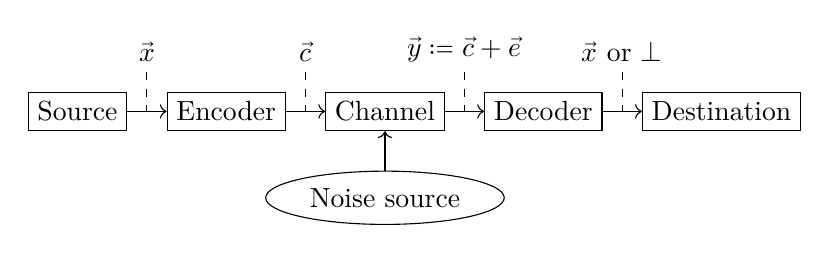
\begin{tikzpicture}[auto, node distance=.5cm]
      \node[draw] (source) {Source};
      \node[draw, right=of source] (encoder) {Encoder} edge[<-] (source);
      \node[draw, right=of encoder] (channel) {Channel} edge[<-] (encoder);
      \node[draw, right=of channel] (decoder) {Decoder} edge[<-] (channel);
      \node[draw, right=of decoder] (destination) {Destination} edge[<-] (decoder);
      
      \node[draw, ellipse, below=of channel] (noise) {Noise source} edge[->] (channel);
      
      \coordinate (source-encoder) at ($(source.east)!0.5!(encoder.west)$);
      \coordinate (encoder-channel) at ($(encoder.east)!0.5!(channel.west)$);
      \coordinate (channel-decoder) at ($(channel.east)!0.5!(decoder.west)$);
      \coordinate (decoder-destination) at ($(decoder.east)!0.5!(destination.west)$);

      \node[above=of source-encoder] (message-1) {\(\vec{x}\)} edge[dashed] (source-encoder);
      \node[above=of encoder-channel] (signal) {\(\vec{c}\)} edge[dashed] (encoder-channel);
      \node[above=of channel-decoder] (noisy-signal) {\(\vec{y} \coloneqq \vec{c} + \vec{e}\)} edge[dashed] (channel-decoder);
      \node[above=of decoder-destination] (message-2) {\(\vec{x}\) or \(\bot\)} edge[dashed] (decoder-destination);
    \end{tikzpicture}
    \caption{Transmitting information over a noisy channel.}
  \end{figure}
\end{frame}

\section{The GPT Cryptosystem}

\subsection{Basic Concepts}

\begin{frame}{Linear Codes}
  \begin{definition}[Linear Code]
    An \([n, k]\)\=/code \(\mathcal{C}\) over a finite field \(\FF\)
    is a \(k\)\=/dimensional subspace of the vector space \(\FF^n\).
    The elements of \(\mathcal{C}\) are called \emph{codewords}.

    \(\mathcal{C}\) is an \([n, k, d]\)\=/code if
    \(d = \min\{\norm{\vec{x} - \vec{y}} : \vec{x}, \vec{y} \in
    \mathcal{C}, \vec{x} \ne \vec{y}\}\) for some norm
    \(\norm{\cdot}\).  \(d\) is called the \emph{minimum distance} of
    the code with respect to \(\norm{\cdot}\).
  \end{definition}
  An \([n, k, d]\)\=/code can correct an error \(\vec{e}\) if and only
  if \[\norm{\vec{e}} \le t \eqqcolon \floor{(d - 1) / {2}}\text.\]
  \(t\) is called the \emph{error\-/correcting capacity} of
  \(\mathcal{C}\).
\end{frame}

\begin{frame}{Generating and Utilizing Linear Codes}
  \begin{definition}[Generator Matrix]
    A full\-/rank matrix \(\mat{G} \in \FF^{k \times n}\) is said to
    be a \emph{generator matrix} for the \([n, k]\)\=/code
    \(\mathcal{C}\) if its rows span \(\mathcal{C}\) over \(\FF\).  In
    other words, if
    \[
      \mathcal{C} = \{\vec{x} \mat{G} : \vec{x} \in \FF^k\}\text.
    \]
    \(\mat{G}\) defines an \emph{encoding map}
    \(f_{\mat{G}}\colon \FF^k \to \FF^n\) given by
    \(\vec{x} \mapsto \vec{x} \vec{G}\).
  \end{definition}
  \begin{enumerate}
  \item A message \(\vec{x} \in \FF^k\) is encoded as
    \(\vec{c} \coloneqq \vec{m}\mat{G} \in \FF^n\).
  \item The codeword \(\vec{c}\) is inflicted by noise and received as
    \(\vec{y} \coloneqq \vec{c} + \vec{e}\) with
    \(\norm{\vec{e}} \le t\).
  \item If an efficient decoding procedure exists for \(\mathcal{C}\),
    \(\vec{y}\) is decoded into \(\vec{x}\).  (Decoding can of course
    be done without an efficient procedure, but will be
    computationally very demanding.)
  \end{enumerate}
\end{frame}

\begin{frame}{The Rank Metric}
  \begin{definition}[Rank Norm]
    Let
    \(\vec{x} \coloneqq \begin{bmatrix} x_1 & \cdots &
      x_n \end{bmatrix} \in \FF_{q^m}^n\) and
    \(\{\beta_1, \ldots, \beta_m\}\) be a basis of \(\FF_q^m\) over
    \(\FF_q\).  For all \(i \in \{1, \ldots, n\}\), we can write
    \(x_i = \sum_{j = 1}^m x_{i, j} \beta_j\) with
    \(x_{i, j} \in \FF_q\).  The \emph{rank norm} \(\normR{\cdot}{q}\)
    is defined as
    \begin{equation}\label{eq:rank-norm}
      \normR{\vec{x}}{q} \coloneqq \rank \begin{bmatrix}
        x_{1, 1} & \cdots & x_{1, m} \\
        \vdots & \ddots & \vdots \\
        x_{n, 1} & \cdots & x_{n, m}
      \end{bmatrix}\text.
    \end{equation}
  \end{definition}
  The rank norm of is independent of the choice of basis and induces a
  metric called the \emph{rank metric} (or \emph{rank distance}):
  \[\dR(\vec{x} - \vec{y}) \coloneqq \normR{\vec{x} -
      \vec{y}}{q}\text.\]
\end{frame}

\subsection{Gabidulin Codes}

\begin{frame}{Generating Gabidulin Codes}
  \Textcite{Gab85} constructed a family of Maximum Rank Distance codes
  over \(\FF_{q^m}\) of length \(n \le m\).  For any
  \(x \in \FF_{q^m}\) and any \(i \in \ZZ\), the quantity
  \(x^{[i]} \coloneqq x^{q^i}\).
  \begin{definition}[Gabidulin Code]
    Let
    \(\vec{g} \coloneqq \begin{bmatrix} g_1 & \cdots &
      g_n \end{bmatrix} \in \FF_{q^m}^n\) with all \(g_i\) independent
    over \(\FF_q\).  (This implies \(n \le m\).)  The \emph{Gabidulin
      code} of dimension \(k\), \(\Gab_k(\vec{g})\), is generated by
    \begin{equation}\label{eq:gabidulin-code-generator}
      \mat{G} \coloneqq
      \begin{bmatrix}
        g_1^{[0]} & \cdots & g_n^{[0]} \\
        \vdots & \ddots & \vdots \\
        g_1^{[k - 1]} & \cdots & g_n^{[k - 1]}
      \end{bmatrix}\text.
    \end{equation}
  \end{definition}
  Gabidulin codes have \(d = n - k + 1\), hence errors of rank
  \(t = \floor{(n - k) / {2}}\) can be corrected in time
  \(\BigOh(d^3 + d n)\).
\end{frame}

\subsection{Description of the GPT Cryptosystem}

\begin{frame}{The GPT Cryptosystem}{System Parameters and Key Generation}
  \structure{System Parameters}
  \begin{itemize}
  \item Choose \(k, n, m \in \NN\) such that \(k < n \le m\).
  \item Define the error\-/correcting capacity
    \(t = \floor{(n - k) / {2}}\).
  \item Choose \(l \in \NN\) with \(l \ll n\).
  \end{itemize}

  \structure{Key Generation}
  \begin{itemize}
  \item Let \(\vec{g} \in \FF_{q^m}^n\) with
    \(\normR{\vec{g}}{q} = n\) and let \(\mat{G}\) be a generator of
    \(\Gab_k(\vec{g})\).
  \item Let \(\mat{S} \in \GL_k(\FF_{q^m})\) and
    \(\mat{P} \in \GL_{n + l}(\FF_q)\).  Note that \(\mat{P}\) is an
    \emph{isometry} in the rank metric.
  \item Let \(\mat{X}_1 \in \FF_{q^m}^{k \times l}\) and
    \(\mat{X}_2 \in \FF_{q^m}^{k \times n}\) with
    \(\rank\mat{X}_2 < t\).
  \item Define the \emph{distortion transformation}
    \[
      \Distort(\mat{G}) \coloneqq
      \mat{S}
      \begin{bmatrix} \mat{X}_1 & \mat{G} + \mat{X}_2 \end{bmatrix}
      \mat{P}\text.
    \]
  \end{itemize}
\end{frame}

\begin{frame}{The GPT Cryptosystem}{Public Key, Encryption, and Decryption}
  \begin{itemize}
  \item The \structure{public key} consists of
    \(\mat{G}_{\pub} \coloneqq \Distort(\mat{G})\) and
    \(t_{\pub} \coloneqq t - \rank\mat{X}_2\).
  \item To \structure{encrypt} \(\vec{x} \in \FF_{q^m}^k\), choose
    \(\vec{e} \in \FF_{q^m}^n\) with
    \(\normR{\vec{x}}{q} \le t_{\pub}\) and compute
    \(\vec{y} \coloneqq \vec{x} \mat{G}_{\pub} + \vec{e}\).
  \item To \structure{decrypt} \(\vec{y} \in \FF_{q^m}^n\), apply the
    decoding procedure for \(\Gab_k(\vec{g})\) to the last \(n\)
    components of \(\vec{y} \mat{P}^{-1}\) to obtain
    \(\vec{x} \mat{S}\), then just multiply by \(\mat{S}^{-1}\).
    \alert{The math works out just nicely}.
  \end{itemize}
\end{frame}

\begin{frame}{The GPT Cryptosystem}{Common Form of the Public Key}
  We simplified and generalized the following theorem due to
  \textcite{Ksh07}.
  \begin{theorem}[GPT Public Key]
    Let \(\mat{G}_{\pub}\) be a public GPT key, and assume that
    \(\rank\mat{X}_2 = t_{\mat{X}_2}\).  Then, there exist
    \(\mat{P}^* \in \GL_{l + n}(\FF_q)\),
    \(\mat{X}^* \in \FF_{q^m}^{k \times (l + t_{\mat{X}_2})}\), and
    \(\mat{G}^*\) which generates an
    \([n - t_{\mat{X}_2}, k]\)\=/Gabidulin code \(\Gab_k(\vec{g}^*)\).
    Furthermore,
    \[
      \mat{G}_{\pub} =
      \mat{S}
      \begin{bmatrix} \mat{X}^* & \mat{G}^* \end{bmatrix}
      \mat{P}^*\text,
    \]
    and \(\Gab_k(\vec{g}^*)\) can correct more than \(t_{\pub}\) errors.
  \end{theorem}
\end{frame}

\subsection{Overbeck's Attack and Loidreau's Reparation}

\begin{frame}{Distinguishing Properties}
  \begin{definition}
    For any \(i \in \NN\), let
    \(\Lambda_i\colon \FF_{q^m}^{k \times n} \to \FF_{q^m}^{i k \times
      n}\) be the \(\FF_q\)\=/linear operator defined as:
    \[
      \Lambda_i(\mat{X}) \coloneqq
      \begin{bmatrix}
        \mat{X}^{[0]} \\
        \vdots \\ \mat{X}^{[i - 1]}
      \end{bmatrix}\text.
    \]
  \end{definition}
  For any code \(\mathcal{C}\) generated by \(\mat{G}\), we denote by
  \(\Lambda_i(\mathcal{C})\) the code generated by
  \(\Lambda_i(\mat{G})\).  \alert{It turns out that \(\Lambda_i\) can
    distinguish Gabidulin codes from random}.
\end{frame}

\begin{frame}{Gabidulin vs.\ Random}
  \begin{lemma}
    Let \(\vec{g} \in \FF_{q^m}^n\) with \(\normR{\vec{g}}{q} = n\).
    For \(i \in \NN\) such that \(i \le n - k - 1\),
    \[
      \Lambda_i(\Gab_k(\vec{g})) = \Gab_{k + i}(\vec{g})\text.
    \]
  \end{lemma}
  On the other hand, if \(\mat{G}\) is a randomly\-/drawn matrix, we
  obtain something quite different.  \Textcite{Ove05, Ove06, Ove08}
  formulated a successful attack against GPT using these properties.
  \begin{lemma}
    If \(\mathcal{C} \subset \FF_{q^m}^n\) is a code generated by a
    random matrix \(\mat{G} \in \FF_{q^m}^{k \times n}\),
    \[
      \dim\Lambda_i(\mathcal{C}) = \min\{n, (i + 1) k\}
    \]
    with high probability.
  \end{lemma}
\end{frame}

\begin{frame}{Reparation by \textcite{Loi17}}
  Crucial to the structural attack against GPT are:
  \begin{itemize}
  \item The distinguishing properties of \(\Gab_k(\vec{g})\) under
    \(\Lambda_i\).
  \item The invariance of \(\mat{P} \in \GL_{n + l}(\FF_q)\) under
    \(\Lambda_i\).
  \end{itemize}
  \Textcite{Loi17} tackled these issues by
  \begin{enumerate}
  \item Letting \(\mat{P} \in \GL_{n + l}(\mathcal{W})\), where
    \(\mathcal{W}\) is a \(\lambda\)\=/dimensional subspace of
    \(\FF_q^m\).
  \item Using \(\mat{P}^{-1}\) to scramble and \(\mat{P}\) to
    unscramble instead of the other way around.
  \end{enumerate}
  This has the effect of \alert{resisting the structural attack} at
  the cost of reducing the error\-/correcting capacity by a factor of
  \(\lambda\).
  \begin{alertblock}{No Structural Exploits}
    Our best attacks against this reparation are \emph{generic}.  The
    state\-/of\-/the\-/art comes from \textcite{GRS13}; we will try to
    formulate the \emph{information set decoding} family of algorithms
    in the rank metric.
  \end{alertblock}
\end{frame}

\section{Decoding Random Codes in the Rank Metric}

\subsection{State-of-the-Art}

\begin{frame}{Support-Trapping Algorithm by \textcite{GRS13}}
  \begin{itemize}
  \item \(\supp(\vec{e}) \coloneqq\) subspace \(\mathcal{E}\) which
    contains each \(e_i\).
  \item Assume \(\normR{\vec{e}}{q} \le w \implies \mathcal{E}\) is
    w.l.o.g.\ \(w\)\=/dimensional.
  \item However, we may need to guess \(\mathcal{E}' > \mathcal{E}\)
    to be able to solve for \(\vec{e}\).
  \item \Textcite{GRS13} showed how to retrieve \(\vec{e}\) in time
    \(\BigOh(q^{w \ceil{m k / {n}}})\) by:
    \begin{enumerate}
    \item Taking \(\mathcal{E}'\) to be of dimension
      \(\ceil{(n - k) m / {n}}\); and
    \item Writing each \(e_i\) in \(\mathcal{E}'\).
    \end{enumerate}
  \end{itemize}
  \begin{alertblock}{An ISD-Inspired Variation}
    Instead of guessing a superspace of \(\mathcal{E}\), we will\---
    analogously to ISD algorithms in the Hamming metric\--- guess a
    subspace that is \enquote{near\-/orthogonal} to \(\mathcal{E}\).
  \end{alertblock}
\end{frame}

\subsection{Information Set Decoding}

\begin{frame}{Intuition Behind ISD in the Rank Metric}
  Instead of guessing a superspace of \(\mathcal{E}\), we guess
  \(\mathcal{V} \le \FF_q^m\) that is
  \begin{enumerate}
  \item \enquote{Near\-/orthogonal} to \(\mathcal{E}\); and
  \item Allows us to solve for each \(e_i\).
  \end{enumerate}
  Assume that
  \begin{itemize}
  \item \(\mathcal{V}\) is \(\zeta\)\=/dimensional.
  \item \(\mat{P} \in \FF_q^{\zeta \times m}\) projects from
    \(\FF_q^m\) to \(\mathcal{V}\).
  \item \(\tilde{\mathcal{V}}\) is a \(p\)\=/dimensional subspace of
    \(\mathcal{V}\), for \(p \in \{0, \ldots, \zeta\}\).
  \item \(\basis{\tilde{\vec{v}}_1, \ldots, \tilde{\vec{v}}_p}\) is a
    basis for \(\tilde{\mathcal{V}}\).
  \end{itemize}
\end{frame}

\begin{frame}{Description of the Algorithm}
  \begin{equation}\label{eq:ISD}
    \{\mat{P} \overbrace{(y_i - {(\vec{x} \mat{G})}_i)}^{e_i} = \sum_{j
      = 1}^p \gamma_{i, j} \tilde{\vec{v}}_j : i \in \{1, \ldots,
    n\}\}
  \end{equation}
  is a linear system over \(\FF_q\) in \(\zeta n\) equations and
  \(m k + n p\) unknowns
  \(\implies \alert{\zeta = \ceil{m k / {n}} + p}\).  Now:
  \begin{enumerate}
  \item Assume \(\normR{\vec{e}}{q} \le w\).
  \item Solve for \(\vec{x}\) in~\eqref{eq:ISD}.
  \item If \(\normR{\vec{y} - \vec{x} \mat{G}}{q} \le w\), then we
    have a successful iteration.  Otherwise, try a new \(\mathcal{V}\)
    along with all \(p\)\=/dimensional \(\tilde{\mathcal{V}}\)'s.
  \end{enumerate}
\end{frame}

\begin{frame}{Complexity Analysis of the Algorithm}{Setting Up the Stage}
  Informally, we need the
  \begin{itemize}
  \item Probability that \enquote{\(w - p\) dimensions} of
    \(\supp(\vec{e})\) come from \(\mathcal{V}^{\perp}\).
  \item Probability that \enquote{\(p\) dimensions} of
    \(\supp(\vec{e})\) come from \(\tilde{\mathcal{V}}\).
  \item The cost of iterating through all \(p\)\=/dimensional
    \(\tilde{\mathcal{V}}\)'s.
  \end{itemize}
  (We can ignore the cost of solving for \(\vec{x}\) as it is a simple
  linear system.)
  \begin{alertblock}{A Counting Argument}
    In order to evaluate the two probabilities, we:
    \begin{enumerate}
    \item Count all \enquote{good} choices; and
    \item Divide that number by the total number of choices for
      \(\supp(\vec{e})\).
    \end{enumerate}
  \end{alertblock}
\end{frame}

\begin{frame}{\(q\)-Binomial Coefficients}{Counting Vector Spaces}
  \begin{definition}[\(q\)-Binomial Coefficient]
    The \emph{\(q\)\=/binomial coefficient} (also called
    \emph{Gaussian binomial coefficient}) is defined by
    \[
      \qbinom{m}{r}_q =
      \begin{cases}
        \frac{(1 - q^m) (1 - q^{m - 1}) \cdots (1 - q^{m - r + 1})}{(1 - q) (1 - q^2) \cdots (1 - q^r)} & r \le m\\
        0 & r > m\text.
      \end{cases}
    \]
    Furthermore, it satisfies
    \[
      \qbinom{m}{r}_q \in \Theta(q^{r (m - r)})\text.
    \]
  \end{definition}
  The \(q\)\=/binomial coefficient counts the \alert{number of
    \(r\)\=/dimensional subspaces of an \(m\)\=/dimensional vector
    space over \(\FF_q\)}.
\end{frame}

\begin{frame}{Complexity Analysis of the Algorithm}{Final Results}
  We can see that the probability of a successful iteration is
  \[
    \qbinom{\zeta}{p}_q \qbinom{m - \zeta}{w - p}_q \qbinom{m}{w}_q^{-1}\text,
  \]
  while the cost of iterating through all \(\tilde{\mathcal{V}}\)'s is
  \[
    \qbinom{\zeta}{p}_q\text.
  \]
  This gives an average complexity of
  \[
    \qbinom{m - \zeta}{w - p}_q^{-1} \qbinom{m}{w}_q \in \Theta(q^{w
      \zeta + p (p + m - \zeta)})\text.
  \]
  \(m > \zeta \implies\) it is minimized when \alert{\(p = 0\)} and
  becomes the same as in~\cite{GRS13}:
  \[
    \Theta(q^{w \ceil{m k / {n}}}).
  \]
\end{frame}

\begin{frame}[allowframebreaks]{References}
  \printbibliography{}
\end{frame}

\end{document}

%%% Local Variables:
%%% mode: latex
%%% TeX-command-extra-options: "-shell-escape"
%%% TeX-engine: luatex
%%% TeX-master: t
%%% End: